\chapter{Shape-Change Termination}

One trouble with size-change termination as described in the previous chapter
is \referToLemma{cycle-reduce}. This lemma makes size-change termination weak
in the sense that the overall shape changes in a given call cycle are
\emph{not} considered, and instead, the calls of any call cycle are constrained
to nonincreasing calls. However, there may be programs that have calls, or even
call cycles, that in terms of size, increase a value for a finite amount of
time, until some condition is met, or as in the case of \D{}, it has some
particular shape.

% TODO: define nonincreasing call to be a call that does not increase a value.

Consider the program in \referToListing{size-change-fail} as an example of a
program for which regular size-change termination is unable to determine the
halting property, while the property itself would seem fairly simple to deduce.
This is a sample program where some value is increased in terms of size in a
call cycle, but only until the value matches a certain shape, the shape
required by a terminal clause.

\begin{lstlisting}[
  label=listing:size-change-fail,
  caption={A terminating program with a call cycle where a value is
  temporarily increased.}]
$f_0$: f a.b.c.d := a
$f_1$: f a := f a.0
f input
\end{lstlisting}

The extension proposed in this chapter is to be able to determine the halting
property for such a class of programs without reducing size of the class of
programs for which size-change termination can already deduce the halting
property.

\section{The class of programs considered}

Before we can speak of extending size-change termination to determine the
halting property for programs in the same class as
\referToListing{size-change-fail}, we need to formally define that class.

Actual conditions in \D{} can only be expressed in terms of patterns in
function clauses. Hence, we disregard programs that rely on equality or size
comparison conditions for termination, since this type of programs will often
already be covered by regular size-change termination, and if not, they at the
very least come down to recursive pattern matching.

As an example of a program where size-change termination is already prevalent,
consider a program that finds the $n^{th}$ Fibonacci number as the one already
presented in \referToSection{d-samples}. The function \mono{fibonacci-aux}
seemingly increases a value until a condition is met, in particular, until we
count one of the arguments down to \mono{0}. However, due to the fact that we
count that we decrease the value of that argument in \emph{recursive} clause of
the \mono{fibonacci-aux} functions, the halting property is certainly already
deducible by regular size-change termination.

Instead, we turn our attention to simpler programs, ones that rely solely on
conditions defined in terms of patterns. Consider again the program in
\referToListing{size-change-fail}. The function \mono{f} has only one terminal
clause, the one that accepts a shape as in \referToFigure{size-change-fail-f0}.
If the function argument has any other shape, i.e. either a shape as in
\referToFigure{size-change-fail-f1-0}, \referToFigure{size-change-fail-f1-1} or
\referToFigure{size-change-fail-f1-2}, then the recursive clause $f_1$ is
chosen. For any argument $b\in\mathbb{B}$, the clause $f_1$ replaces the
right-most child of the value, which is always \mono{0}, with a node.

For instance, the smallest possible argument $b\in\mathbb{B}$ is \mono{0}.  If
passed such a value, $f_1$ transforms it into a value that has a shape that
corresponds to \referToFigure{size-change-fail-f1-1}, which in turn transforms
the value into one that matches \referToFigure{size-change-fail-f1-2}, which in
turn transforms the value into one that matches
\referToFigure{size-change-fail-f0}, i.e. the terminal clause. What's more,
there are infinitely many other values that will match the shape
\referToFigure{size-change-fail-f1-1}, and for each of them, the clause $f_1$
will transform them into values that match
\referToFigure{size-change-fail-f1-2}, which will transform them into values
that match \referToFigure{size-change-fail-f0}.

\includeFigure{size-change-fail-f0}{The shape that the clause $f_0$ in
\referToListing{size-change-fail} will accept.}

\begin{figure}[htbp!]
\begin{minipage}{0.3\linewidth}
\centering
\includegraphics{figures/size-change-fail-f1-0}
\caption[]{The pattern \mono{0}.}
\label{figure:size-change-fail-f1-0}
\end{minipage}
\begin{minipage}{0.3\linewidth}
\centering
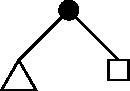
\includegraphics{figures/size-change-fail-f1-1}
\caption[]{The pattern \mono{a.0}.}
\label{figure:size-change-fail-f1-1}
\end{minipage}
\begin{minipage}{0.3\linewidth}
\centering
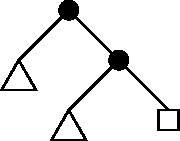
\includegraphics{figures/size-change-fail-f1-2}
\caption[]{The pattern \mono{a.b.0}.}
\label{figure:size-change-fail-f1-2}
\end{minipage}
\end{figure}

We shall henceforth say that a clause such as $f_1$ changes the shape of any
argument $b$ to \emph{eventually} match the shape corresponding to a pattern of
the terminal clause $f_0$. The task then becomes to determine for each call
cycle in a program whether it changes the shape of the argument to eventually
match some terminal clause.

\section{Prerequisites}

Before we continue with this extension we can make a few important observations
based on the semantics of function clauses in \D{}.

\subsection{Deducing leafs}\label{section:extend-deducing-zero}

The \mono{.} operator in the patterns of function clauses in \D{} is
right-associative. Hence, a pattern of the form \mono{a.b.c.d} is the same as
\mono{a.(b.(c.d))}. This implies that we can always construct a parenthesized
version of any valid pattern, indeed this is required to keep the syntax
unambiguous. This associativity can be overridden by the conventional use of
parentheses, e.g. a pattern like \mono{(a.b).c.d} is the same as
\mono{(a.b).(c.d)}. 

Consider the function defined in \referToListing{deducing-zero}. If $f_0$ and
$f_1$ both fail to accept some argument $b\in\mathbb{B}$, then $b$ must match
the pattern $0\cdot b'$, where $b'\geq 0$, that is, on entry to $f_2$, \mono{d}
is \emph{always} bound to \mono{0}, and \mono{e} is always bound to some
$b'\geq 0$.

\begin{proof} Otherwise, either $f_0$ or $f_1$ would've matched. \end{proof}

\begin{lstlisting}[label=listing:deducing-zero,
  caption={A sample program for showing 0-deduction.}]
$f_0$: f 0 := 0
$f_1$: f (a.b).c := 0
$f_2$: f d.e := 0
\end{lstlisting}

Such a deduction is not always unambiguous as the function in
\referToListing{deducing-zero-fail} exhibits. Here, if $g_0$ and $g_1$ both
fail to accept some argument $b\in\mathbb{B}$, then the shape of $b$ is either
$0\cdot b'$ or $b'\cdot 0$ where $b\geq 0$. However, one thing is certain, and
that is that $b$ can't have the shape $b'\cdot b''$ where $b'>0$ and $b''>0$.

\begin{lstlisting}[label=listing:deducing-zero-fail,
  caption={A sample program where 0-deduction is ambiguous.}]
$g_0$: g 0 := 0
$g_1$: g (a.b).(c.d) := 0
$g_2$: g e.f := 0
\end{lstlisting}

\section{Shape-change termination}

By \referToCorollary{pattern-shape}, a pattern is a shape specification. By
\referToDefinition{unary-clause}, all clauses are unary, and hence a clause can
be said to specify a shape. By \referToDefinition{function-tuple}, a function
call contains a finite list of clauses.

\begin{theorem} Any function specifies a finite number of disjoint
shapes.\end{theorem}

\begin{proof} The shapes specified by a function are derived from the patterns
of its clauses.\end{proof}

Instead of constructing a call graph with every clause in a program as a node,
we construct a call graph with every shape of every function call as a node.
This builds upon the idea that there is a finite number of disjoint shapes
deducible from the clauses of any function definition, which renders the number
of nodes in the graph finite. The number of shapes for any one clause may vary,
and hence there will be multiple edges from caller to its callees, rather than
one edge to the first clause of the callee as seen with regular size-change
termination.

The nodes are iteratively derived starting with the initial clause $c_{main}$,
drawing the edges and callee shapes as function calls are encountered, i.e. we
use an exploration technique to build the graph.

\subsection{Annotation}

In the sections that follow we'll make use of an extended call graph syntax.
The intent of the call graphs in this chapter is to show how a shape changes in
a control transition from source to target. Indeed, the call graphs are no
longer call graphs but \emph{shape change graphs}.

\subsubsection{Success \& fail transitions}

There no longer needs to be drawn a distinction between the two since a value
of some shape will match exactly one choice. In some cases, where a deduction
of a value is fairly evolved this clause may be deduced, in other cases, the
success \& fail transitions will be regarded as one and the same. 

\subsection{Patterns and shapes}

By \referToDefinition{shape}, the only shape we may assume for any unknown
$b\in\mathbb{B}$ is the triangle.

For any unknown value, we may assume only one shape, the tree. Hence, given a
program like the one in \referToListing{size-change-fail}, we start analyzing
the function \mono{f} by assuming nothing about the input argument, i.e.
annotating it with a $\bigtriangleup$. The value may match either clause, but
it will match exactly one. If the value matches a clause, that indicates that
the value has a certain shape, indeed this is what a pattern declaration is --
a shape specification, or a requirement, if you wish. The position of the
clause enclosing the pattern wrt. to other clauses can be used to reduce the
singleton set of possible values to a set containing multiple, more concrete
shapes. All in all, multiple clauses may be chosen, and as already discussed
for clause $f_1$, multiple shapes can be deduced for a given clause, we
consider \emph{all} possible shapes.
\referToFigure{size-change-fail-shape-init} illustrates this initial step.

\includeFigure{size-change-fail-shape-init}{Initializing shape analysis for the
program in \referToListing{size-change-fail}.}

\subsubsection{Deducing shapes from patterns}

Shape deduction is an iterative, and initially non-terminating process for any
non-terminating program. We begin by introducing the rules that allow us to
deduce shapes from patterns and call sequences, and make the method terminating
at a later stage.

The method itself builds upon the idea that the sort of iterative pattern
matching that goes on when a function call is made, can be used to deduce
information about the shape of the value. Here, both failure to match a series
of patterns as well as the success to match some pattern eventually are useful.
In particular, the series of failed pattern matches indicate which shapes the
value \emph{does not} have, which in turn allows us to assemble a finite set of
shapes, one of which \emph{must} match the value\footnote{If a pattern matches
a value then the value matches the pattern, and vice versa.}. We use this
information as we look at the subsequent patterns where patterns themselves
might not be descriptive enough. For instance, consider how failure to match a
node allowed us to deduce a leaf, although the subsequent pattern itself
indicated simply a tree shape in \referToSection{extend-deducing-zero}.

\begin{lemma}\label{lemma:extend-first-clause} If a value $v$ matches the
pattern $p$ of the first clause $c$ of a function declaration $f$, then only
one possible shape of $v$ is known, indeed it is the one represented by
$p$.\end{lemma}

\begin{proof} The first clause of a function declaration is the first clause
considered by \D{}'s runtime when a function call is made. No \emph{other}
clauses, and hence patterns, have been attempted at this point. There is
therefore no information about the shape of the value other than $p$ itself.
Furthermore, if $v$ matches, then it certainly has the shape indicated by $p$,
otherwise, $v$ wouldn't have matched $p$.\end{proof}

The following are a few definitions and lemma are useful when talking about
shapes.

\begin{definition} Given two shapes, $A$ and $B$, we say that they are disjoint
if the sets of values matched by $A$ and $B$ are disjoint.\end{definition}

\begin{definition} Given two sets of shapes, $X$ and $Y$, we let the operation
$X\Cup Y$ denote an operation where the two sets are joined into one, and the
pairs of shapes that are not pairwise disjoint in the final set are joined with
each other such that if $\exists\ s_1,s_2\in X\Cup Y : s_1\curlyvee s_2$, then
$s_1$ is removed from $X\Cup Y$.  \end{definition}

\begin{lemma}\label{lemma:extend-finite-converse} Given a shape, there is a
finite number of disjoint shapes that are disjoint with that shape.\end{lemma}

\begin{proof} A shape in \D{} is recursively defined in terms of an unlabeled
binary tree, where neither nodes nor leafs have labels, and it is the nodes and
leafs themselves that constitute a ``shape'' together with trees, that match
either trees, nodes or leafs.

Given a shape $A$, there is a corresponding shape $B$ for every leaf, and every
node in $A$, such that $A$ and $B$ are disjoint. In particular, for every leaf
in $A$, $B$ can be given a node with two trees as children, and for every node
in $A$, $B$ can be given a leaf. In either case, $A$ and $B$ end up being
disjoint. What's more, every $B$ is concerned with a different leaf or node,
and no leaf or node in $A$ is ever replaced by a tree, this indicates that all
the shapes $B$ are disjoint wrt. one another as well. The parts in shape $A$
that remain untouched are the trees and there are no converse constructs to trees
as they match both trees, nodes and leafs.

Since in any given shape there is a finite number of nodes and leafs, any shape
has a finite number of disjoint shapes that are disjoint with that shape.
\end{proof}

The following lemma indicates that for any function call there will finitely
many shape branches.

\begin{lemma}\label{lemma:extend-clause-finite} Every pattern in a function
definition, if matched, indicates that the value has one of a finite number of
disjoint shapes.\end{lemma}

\begin{proof} Any pattern is a shape specification, hence, for single-clause
functions this is true due to \referToLemma{extend-first-clause}.

Given a multiple-clause function with two consecutive clauses $c_1$ and $c_2$
with patterns $p_1$ and $p_2$, the presence of $p_1$ reduces the space of
values which can reach $p_2$. Let $\overline{X}$ denote the pairwise disjoint
set of shapes that are disjoint with the shape defined by $p_1$. If $p_1$ fails
to match, then the incoming value must have one of the shapes in
$\overline{X}$, and by the definition of \D{}, any such shape must be accepted
by exactly one of the consecutive clauses. Let $Y$ denote the set of shapes
defined by $p_2$. Then, if $p_2$ matches followed by $p_1$ failing to match,
the shape of the incoming value will be in the set $\overline{X}\Cup Y$.

Since $\overline{X}$ and $Y$ are finite sets by
\referToLemma{extend-finite-converse}, the $\overline{X}\Cup Y$ must be finite
as well.\end{proof}

\section{A description}

\subsection{Relationship between value shape and bound variables.}

\subsection{Shape transitions}

Actual shape transitions occur within the body of a clause.

\subsubsection{Nested function calls}

Unlike regular size-change termination we won't disregard the outcome of nested
function calls, but instead consider the shape shifting that we can deduce from
such calls. Rather intuitively, an expression evaluation terminates if all of
the nested function calls terminate. Hence, for any expression it would require
to start with the ``deepest most'' nested call and work our way up the call
stack from there.

\subsubsection{Between calls}

Consider a unary clause $c$ with a pattern specification $p$ and expression
$x$. Assume that the pattern $p$ matches some unknown value $v$ and the
expression $x$ is hence evaluated with some variables $N$ bound to pairwise
disjoint values, which are strict subsets of $v$, or $v$ itself. Due to
\referToLemma{extend-clause-finite}, when $x$ is evaluated there is a finite
set of value shapes that we've deduced for $v$ due to the fact that it matched
$p$. The variables in the set $N$, without further details, can only be assumed
to all be trees.

When a nested function call is encountered in $x$ we compute a \emph{safe}
shape approximation of all the arguments to the function before considering
what shape shift the actual call might bring about, not least because that
depends on the approximation of the shapes of the arguments.

Any function call argument in \D{} is an expression. An expression is a nested
construction of either concrete values, bound variables or nested function
calls. Given concrete values, and what we've thus far said about the variables
bound in $c$, we can deduce the most concrete shape specification without
knowledge of what the initially unknown $v$ is.

However, nested function calls, again complicate the matters, indeed because
that implies that the shape of the nested function call has to be determined
\emph{before} the shape of the parent function call can be determined. We
could've ignored nested function calls and merely safely assumed the shape of
the value returned by the call was a tree, but that would've been rather
useless to the derivation of the shape returned by clause $c$. Instead, we
follow this stack of nested function calls in an expression (without actually
following the calls), and eventually a base function call that has no function
calls in its arguments. Assume we've reached that nested function call and wish
to determine the halting property for that particular call.

With the finite set of shapes for the arguments we consider the disjoint shapes
of the call destination, and hence determine which clauses may be taken. Note,
of course, that this might be \emph{all} the clauses of the called function.

We repeat this process, branching out in all the possible shapes and clauses
taken. We certainly terminate whenever a value is passed to a terminating
clause. The question hence is what do we do when we reach a loop.

A loop in this case is a shape shifting loop, where a value of a certain shape
input into a certain function leads to a call cycle that \emph{seemingly}
retains the shape of the value. At runtime, if this call cycle is taken, it is
certain that the change that has occurred in the value, if any, has happened in
one of the triangles of the shape specification, since otherwise the shapes
wouldn't have matched and the cycle wouldn't have occurred.

Such cases is where original size change termination comes in handy. If despite
retaining the shape, value is actually decreased in every iteration of the
cycle, the triangle eventually reduces to \mono{0}. 

A function call can at most possibly shift the shape to any of the possible
shapes in a given function.

\section{Termination \& Soundness}

\begin{lemma}\label{lemma:extend-function-finite-shape} Any function
declaration accepts a finite number of shapes for every parameter.\end{lemma}

\begin{proof} Any function in \D{} consists of a finite number of clauses and
by \referToLemma{extend-clause-finite}, every clause accepts a finite number of
shapes for every parameter.\end{proof}

\begin{lemma}\label{lemma:extend-any-function-any-value} Any function accepts
any valid \D{} value as any parameter.\end{lemma}

\begin{proof} Follows from the semantics of \D{}.\end{proof}

\begin{definition} A shape transition source and target are different from a
function call source and target in that a function function may elicit one of
several shape transitions.\end{definition}

\begin{lemma}\label{lemma:extend-any-call-targets} Any possible function call in a program has at least one and at
most all of the shapes of a target function as its shape transition
targets.\end{lemma}

\begin{proof} By \referToLemma{extend-any-function-any-value} any value is
matched by at least one of the shapes of a given function. Any value matches
the triangle shape, and by \referToTheorem{d-all-patterns-all-shapes}, the
patterns for a particular parameter in summation can match any value, i.e. in
total correspond to the triangle shape.\end{proof}

\begin{theorem} A shape shift network can be constructed for any valid program
in finite time.\end{theorem}

\begin{proof} Any given program has a finite number of functions. By
\referToLemma{extend-function-finite-shape} the program may hence initially be
considered as finite forest of shapes. Furthermore, by
\referToLemma{extend-any-call-targets} any pair of shapes can be directly
connected by at most one directed edge. Hence, the said forest has a finite
number of edges. The algorithm is sound if all the edges possibly taken by an
executing program are in place when it terminates.  Hence, if we terminate the
branches of the algorithm whenever they reach a terminal clause or enclose a
loop, eventually the algorithm must terminate.\end{proof}


When a function call is made, a list of expressions, each consisting of nested
constructions of concrete values, bound variables and nested function calls, is
evaluated. For each such call, for each expression in the argument list, we
would like a relationship to be drawn between the target input arguments (for
which we already have some shape information) 


\includeFigure{size-change-fail-shape-done}{Nice}



If there is a cycle where we start from one of the disjoint shapes and come
back to that shape, then the change must've occurred in one of the triangles.
If the value was not decreased (size change termination), then the value
must've been increased, or remained unchanged, and this is an infinite loop.


\begin{proof} Otherwise, there wouldn't have been a loop. This is because the
shapes are disjoint, so a change in a triangle can by no means make the value
match another shape, otherwise the shapes indeed are \emph{not} disjoint.
\end{proof}





\newpage

\section{Notes}

Size change termination is indeed an abstraction of what we would like to do.
Given that $p_0\curlyvee p_1$, we know that if any 


A program can be rewritten into a single function where an extra parameter is
added to each function, to distinguish the functions and each function gets a
number of auxiliary parameters which are ignored in general. This way, a
program of various functions can be transformed into a program consisting of a
single function with many clauses, subsets of which represent the individual
functions of the original program.

The problem is thus reduced to checking the halting property for some single
arbitrary function.

Any function has a number of clauses, at least one. Any terminating program has
at least one terminal clause. The point of checking the halting property is
hence to deduce that any possible recursive clause that is taken, alters the
shape of its arguments in such a way that the call cycle eventually reduces the
value towards one, or several of the base cases.

The benefit of this method over original size change termination is that it
allows for some control transitions to increase values, as long as the overall
cycle size and shape mutation goes towards a some base case.

As much information about the shape of the (changing) value has to be withkept
across calls, unlike original size-change termination that allows to discard
shape information from the previous clause.

Next, we make the observation that several functions may participate in a call
cycle.  and in particular, a subset of the recursive clauses may participate in
a call cycle. The call cycle describes a terminating loop if every control
transition is nonincreasing and at least one is increasing, or the loop shape
shifts one of the values towards a base of one of the participating functions.

\subsection{Recursive and terminal clauses}

\begin{lemma}
A program terminates if all the functions terminate.
\end{lemma}

\begin{proof} Assume for the sake of contradiction that this is does not hold.
That would imply that one of \D{}'s primitives does not terminate, which is
absurd.  \end{proof}

\begin{lemma} A function terminates if all the recursive clauses of the
function definition participate in call cycles that shape shift the input value
towards a terminal clause of the function definition after each iteration.
\end{lemma}

\begin{proof}

\end{proof}


If the value is decreased, the shape distortion need not be withkept since the
shape information that is deducible from here is by no means useful for call
cycle analysis, only size decrease is.

\begin{lstlisting}
$c_0$: count x 0 := x
$c_1$: count x y.z := count (count 0.x y) z
\end{lstlisting}

\begin{lstlisting}
f ((0.a).(0.b)).(0.(0.c)) := 
f a := f a.0
\end{lstlisting}

\begin{verbatim}
equal x y := n-equal (normalize x) (normalize y)
n-equal 0 _._ := 0
n-equal _._ := 0
n-equal 0 0 = 0.0
n-equal a.b c.d = and (n-equal a c) (n-equal b d)
\end{verbatim}

Let $A$ denote the set of values that $p_2$ can
match without regard to $p_1$, let $B$ denote the set of values that $p_1$ can
match, and let $C$ denote the set of values that $p_2$ can come to match if
$p_1$ failed. Since $p_1\curlyvee p_2$, then we know that $B\subset A$,
$C\subset A$, $B\cap C=\emptyset$ and $C=A-B$.



We say that a value "has" a shape and "it is of" a shape.
